% !TEX root = ./thesis.tex

\chapter*{\textbf{Supplementary analysis of land use change in Monteregie \\ \hspace{1em}}}
\addcontentsline{toc}{chapter}{Appendix 4: Supplementary analysis of land use change in Monteregie}

\setcounter{chapter}{5}
\setcounter{table}{0}
\setcounter{figure}{0}

%----------------------------------------------------------------------------------------------------------------

% Figures: values

% Clustering moved to appendix

% PCA
\begin{figure}[h!]
\makebox[\textwidth]{
  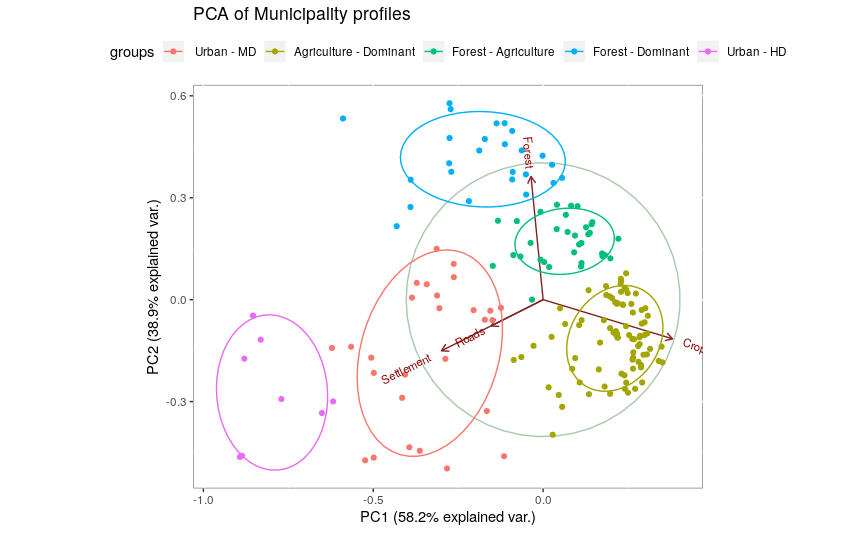
\includegraphics[width=0.8\textwidth]{thesis/figures/PCA_data_profiles.png}
}
\caption{Ordination of land use data (proportions) for municipalities.}
\label{fig:PCAvals}

% MAP
\makebox[\textwidth]{
    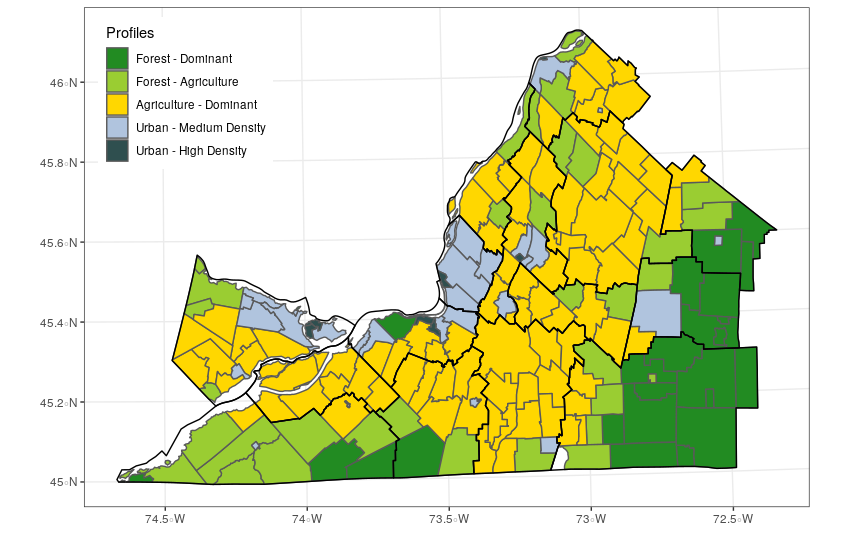
\includegraphics[width=0.8\textwidth]{thesis/figures/profiles_land_use.png}
}
\caption{Geographical distribution of the 5 profiles identified in figure \ref{fig:PCAvals}.}
\label{fig:mapvals}
\end{figure}

% Figures: Transitions

% PCA
\begin{figure}[h!]
\makebox[\textwidth]{
  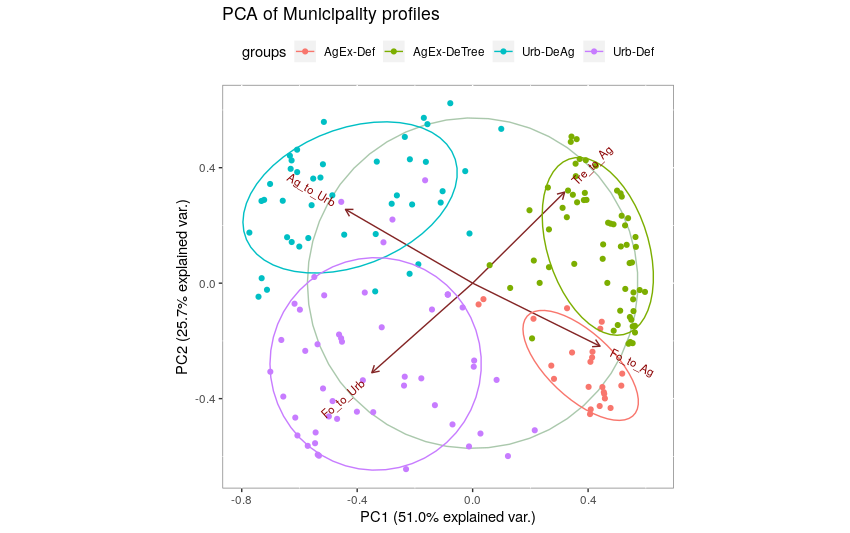
\includegraphics[width=0.8\textwidth]{thesis/figures/PCA_trans_profiles.png}
}
\caption{Ordination of land use transition data for municipalities.}
\label{fig:PCAtrans}

%MAP
\makebox[\textwidth]{
    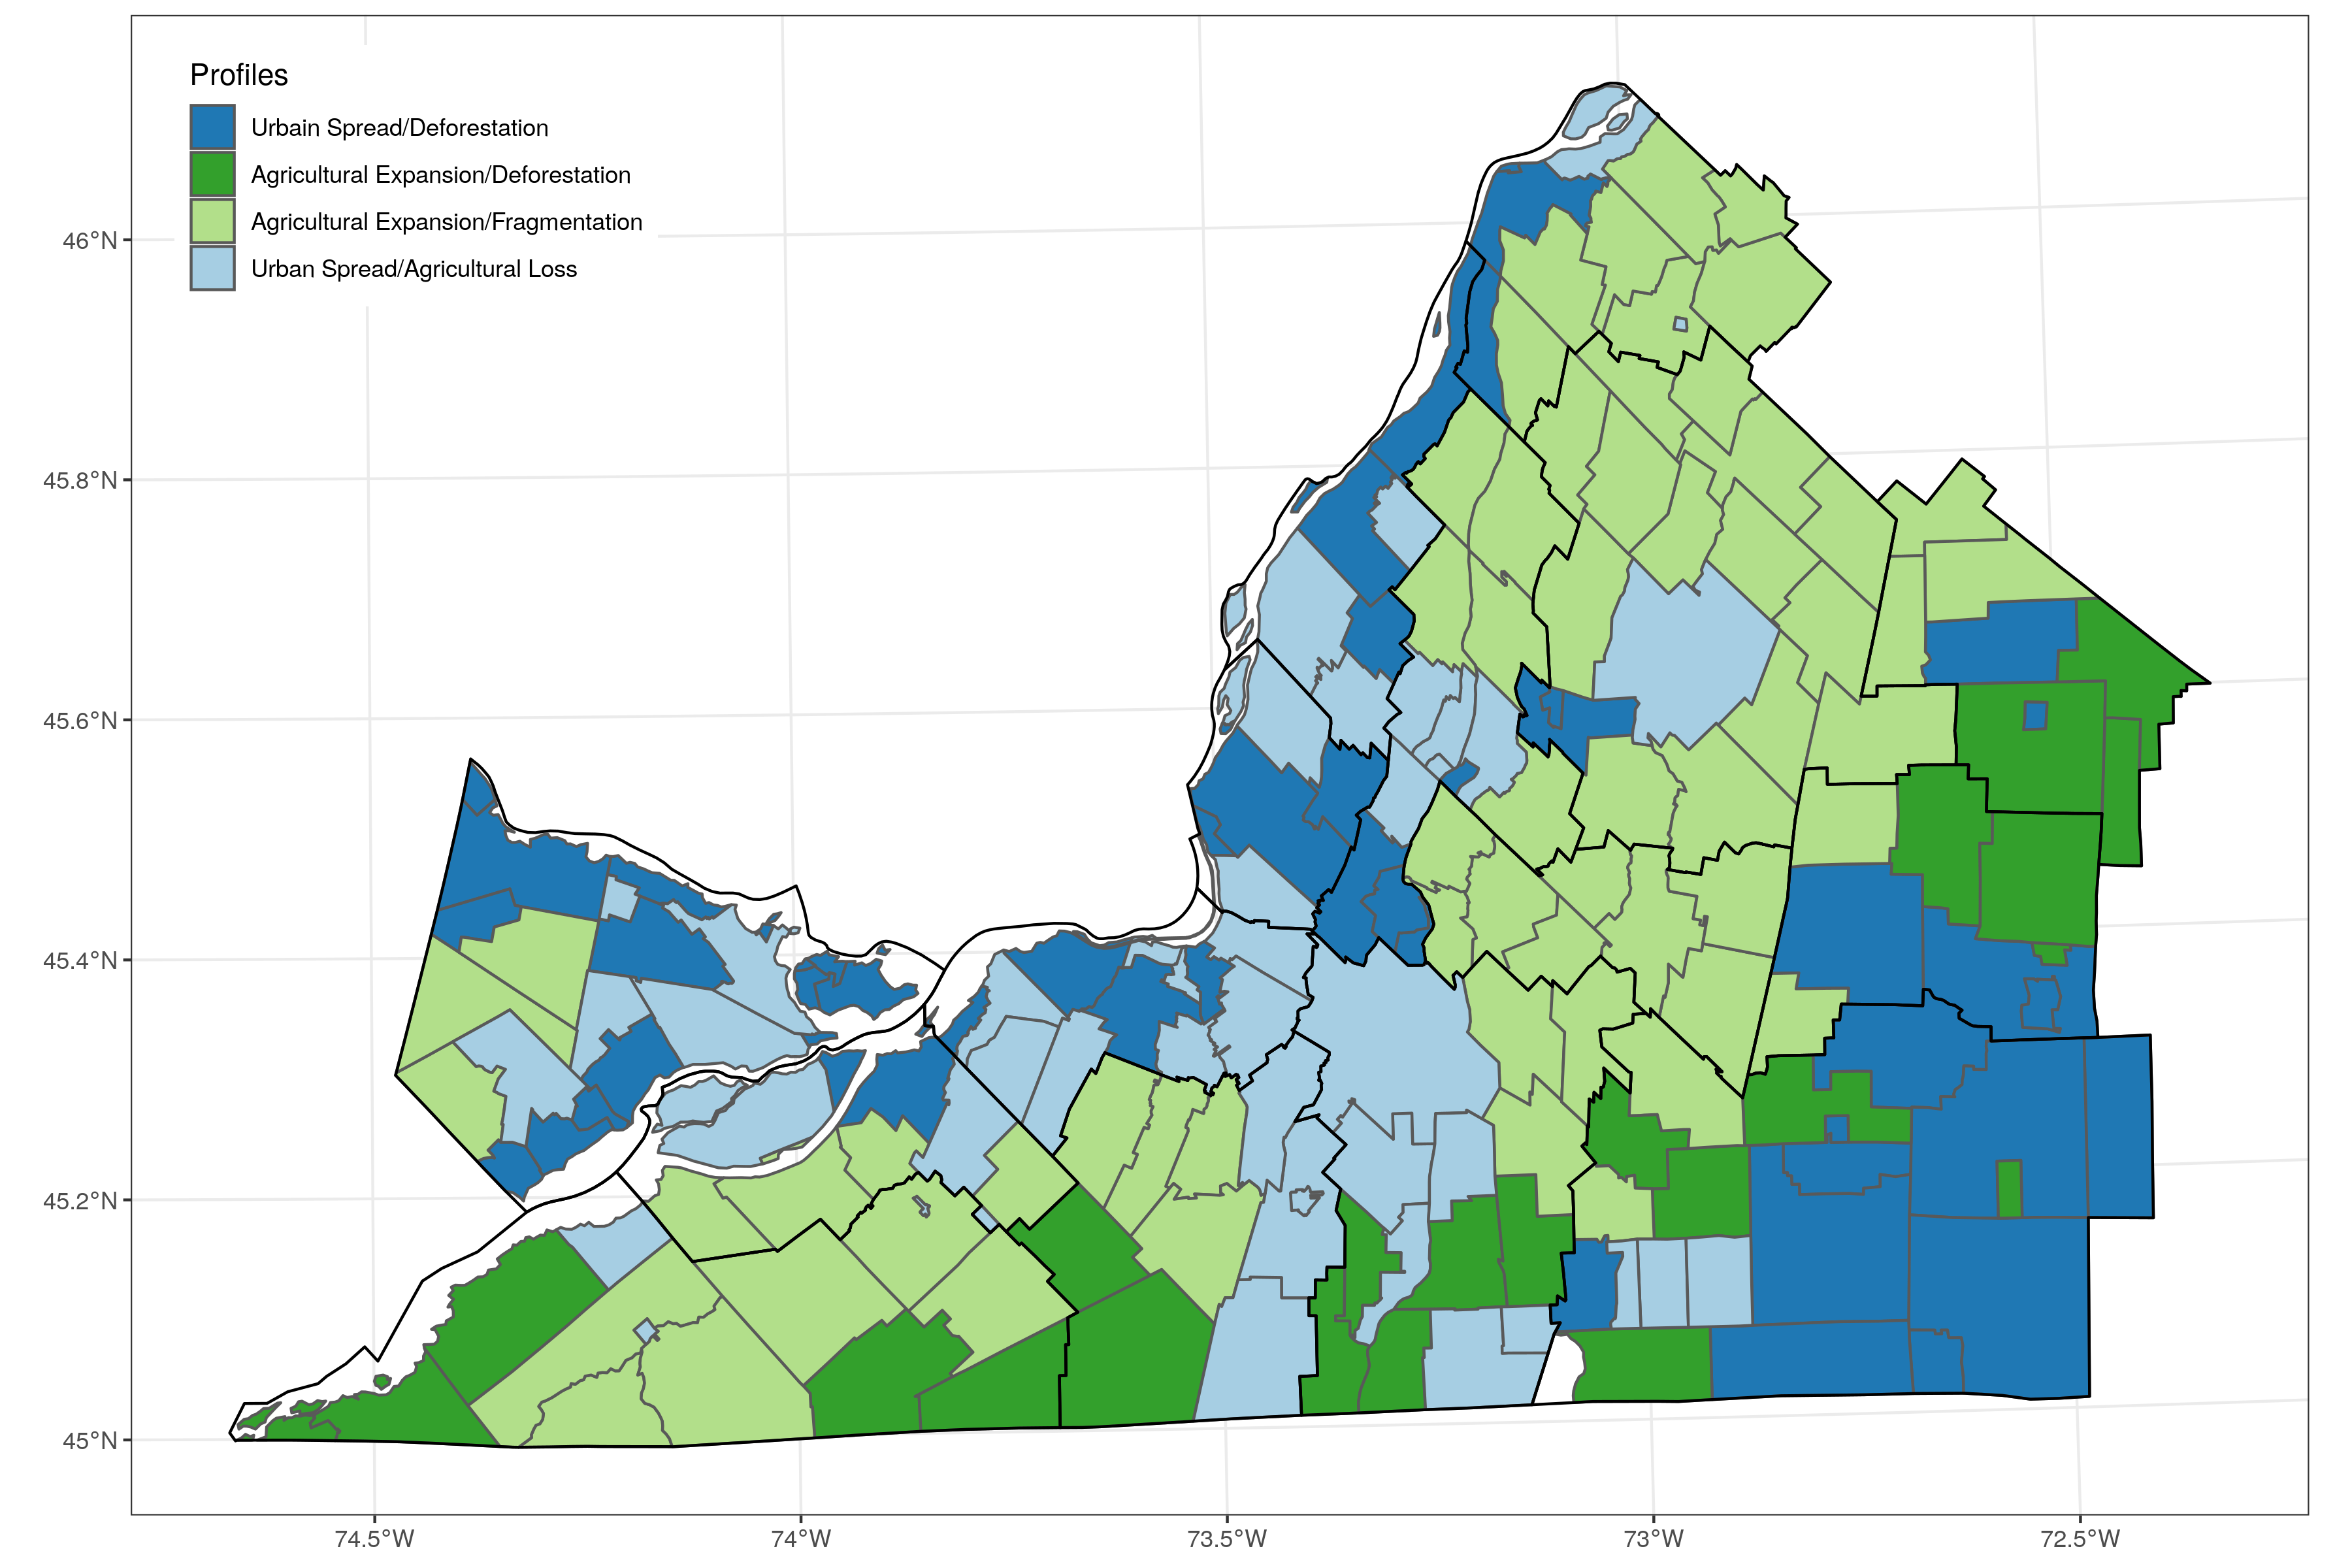
\includegraphics[width=0.8\textwidth]{thesis/figures/transition_prof_map.png}
}
\caption{Geographical distribution of the 4 change profiles identified in figure \ref{fig:PCAtrans}.}
\label{fig:maptrans}
\end{figure}

\clearpage